\chapter{Programmierung der Firmware} \label{ch:Firmware}

\section{Genutzte Applikationen und Webseiten}

Im Rahmen der Durchführung der Maturaarbeit wurden eine Vielzahl von Applikationen und Webseiten genutzt, die den Arbeitsprozess massgeblich unterstützten und die Umsetzung der verschiedenen Projektteile ermöglichten. %Zu den wichtigsten Tools gehörten sowohl Software-Anwendungen als auch Online-Plattformen, die jeweils eine spezifische Funktionalität erfüllten und zur Effizienzsteigerung beitrugen.

Zunächst wurde GitHub\cite{github} als zentrale Plattform für die Versionskontrolle und Zusammenarbeit verwendet. GitHub ermöglichte das einfache Verwalten von Code-Versionen, das Teilen von Projektdateien mit anderen Mitwirkenden und das Verfolgen von Änderungen im Projektverlauf. Die Integration von GitHub in die Entwicklungsumgebung erleichterte die Zusammenarbeit und die Synchronisation zwischen verschiedenen Geräten. 

Für die Entwicklung und das Testen von Softwareanwendungen so wie das Verwenden von Git wurde das Betriebssystem Ubuntu\cite{ubuntuWSL} eingesetzt. Dieses Betriebssystem wurde vom Betreuer dieser ausdrücklich für die Weiterentwicklung der Firmware und dem Versionsaustausch empfohlen. Die Verwendung von Windows Subsystem for Linux (WSL)\cite{ubuntuWSL} ermöglichte es, eine Linux-Umgebung auf einem Windows-System zu betreiben, wodurch die Nutzung von Linux-Tools und -Befehlen innerhalb von Windows möglich wurde. Dies stellte eine effiziente Lösung für die plattformübergreifende Entwicklung dar.

Für die eigentliche Programmierung und Entwicklung wurde Visual Studio Code (VS Code)\cite{microsoftstore} als Code-Editor eingesetzt. Visual Studio Code bietet durch eine Vielzahl von Erweiterungen (Extensions) eine flexible und leistungsfähige Arbeitsumgebung. Insbesondere die Unterstützung für verschiedene Programmiersprachen, die Möglichkeit zur Code-Vervollständigung, das Debugging und die Integration von Git machten VS Code zu einem unverzichtbaren und starken Werkzeug.

Zur Analyse und Konfiguration von Drohnenflugsteuerungen wurde der Betaflight Configurator\cite{betaflightapp} verwendet. Diese Anwendung ermöglicht die Anpassung zentraler Flight-Controller-Einstellungen sowie das präzise Feintuning von Drohnenparametern, die für eine vollständige Konfiguration und Flugfähigkeit der Drohne unverzichtbar sind. Die App erleichterte das Testen und Optimieren der Drohnensteuerung sowie die Datenanalyse.

Für die allgemeine Recherche und das Sammeln von Informationen spielte die Websuche eine zentrale Rolle. Sie half dabei, schnell auf relevante Artikel, technische Dokumentationen und Lösungen für auftretende Probleme zuzugreifen.

Weiterhin wurden Videos als Lernressourcen genutzt. Viele komplexe technische Aspekte, wie das Einrichten von Entwicklungsumgebungen oder das Verständnis von Programmiersprachen, wurden durch Tutorials und Anleitungen in Videoform vertieft.

Abschliessend wurde TeXstudio\cite{texstudio} als Texteditor für die Erstellung der Maturaarbeit verwendet. TeXstudio ist eine beliebte LaTeX-Umgebung, die eine benutzerfreundliche Oberfläche und zahlreiche Features für die effiziente Arbeit mit LaTeX-Dokumenten bietet. Besonders die umfassende Unterstützung von LaTeX-Befehlen erleichterten das Erstellen und Formatieren des Dokuments.

%Die Kombination dieser Applikationen und Webseiten ermöglichte eine effiziente und gut strukturierte Umsetzung der Maturaarbeit und trug entscheidend zum Erfolg des Projekts bei.


\begin{comment}
\section{Analyse der Daten}\label{sec:Tests}

Ziel der Versuche war es, die Neigungswinkel der Drohne in den Achsen \textit{Pitch} und \textit{Roll} zu messen und die entsprechenden Sensordaten zu analysieren. Für die Untersuchungen wurden systematisch festgelegte Neigungswerte in Grad für die Achsen Pitch und Roll verwendet. Diese Variation diente dazu, die Auswirkungen auf die Flugausrichtung der Drohne zu erfassen. Die gemessenen Sensordaten aus den Achsen \(x\), \(y\) und \(z\) wurden aufgezeichnet, um Rückschlüsse auf die Stabilität und das Verhalten der Drohne in unterschiedlichen Neigungssituationen zu ziehen.

\vfill
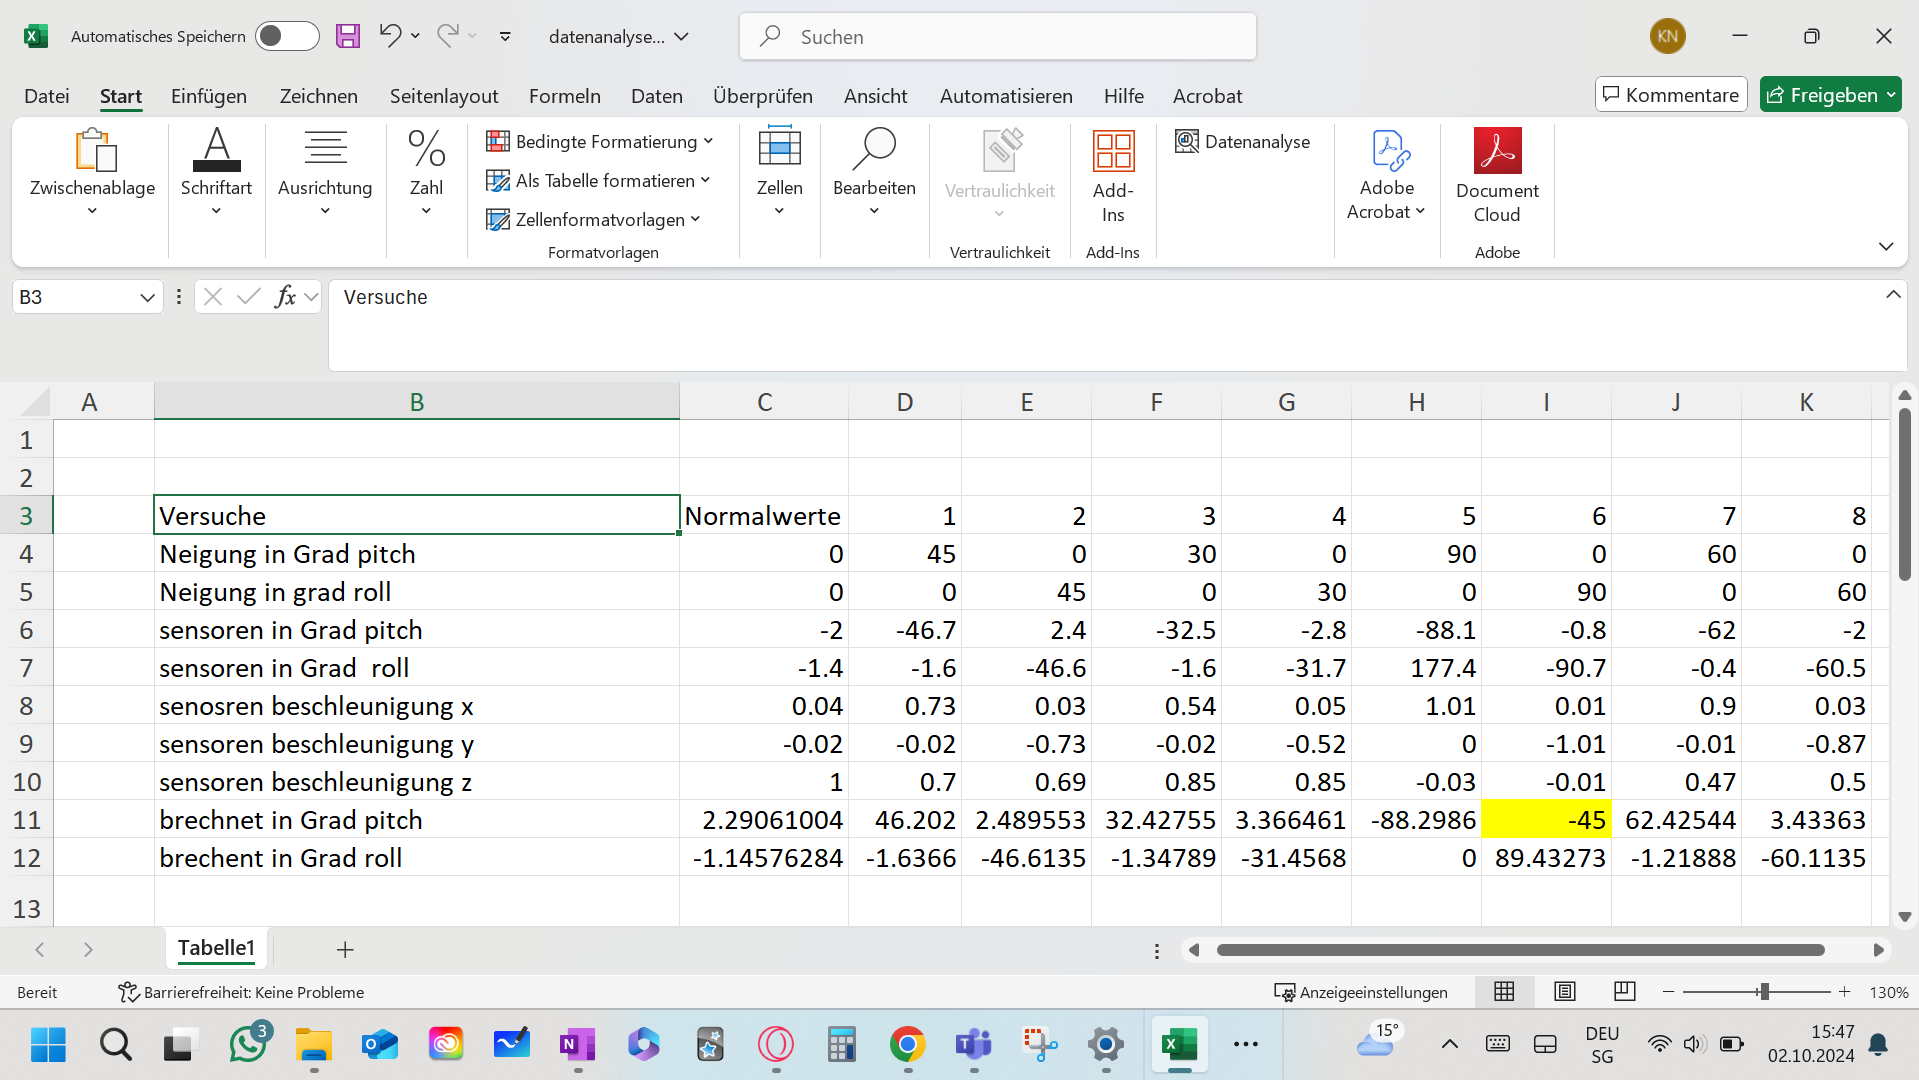
\includegraphics[height=0.3\textheight]{Datenanalyse.png} \vfill
Die ganze Exceltabelle ist auf \href{https://github.com/colordash/Drohne_Project/blob/main/datenanalyse.xlsx}{github} zu finden. 

\subsection{Spalten}
\begin{itemize}
	\item \textbf{Spalte C (Normalwerte)}: Diese Spalte zeigt die theoretischen oder erwarteten „Normalwerte“, also die Werte, die als Standard oder Referenz für die Drohne definiert sind. Diese werden mit den Werten der verschiedenen Versuche (Spalten D bis K) verglichen.
\item\textbf{Spalten D bis K}: Diese Spalten repräsentieren die gemessenen Werte aus acht verschiedenen Versuchen (1 bis 8).
\end{itemize}
\subsection{Zeilen}\begin{itemize}
	\item \textbf{Neigung in Grad pitch (Zeile 4)}: Die Neigung der Drohne in der „Pitch“-Achse, die ihre Vorwärts- oder Rückwärtsneigung beschreibt.
	\item \textbf{Neigung in Grad roll (Zeile 5)}: Die Neigung der Drohne in der „Roll“-Achse, die beschreibt, wie stark die Drohne nach links oder rechts geneigt ist.
	\item \textbf{Sensoren in Grad pitch/roll (Zeilen 6 und 7)}:Diese Zeilen zeigen die gemessenen Daten der Sensoren, die die Neigung in Grad in Pitch (vorwärts/rückwärts) und Roll (links/rechts) erfassen.
	\item \textbf{Sensoren Beschleunigung x/y/z (Zeilen 8 bis 10)}:Diese Zeilen enthalten die gemessenen Beschleunigungswerte der Drohne entlang der drei Achsen (x, y, z), welche die Bewegungen in verschiedene Richtungen anzeigen.
	\item \textbf{Berechnete Werte (Zeilen 11 und 12)}:Die berechneten Winkel in Grad für Pitch und Roll basieren auf den gesammelten Sensordaten. Diese Werte sind das Ergebnis einer mathematischen Berechnung oder Schätzung, die möglicherweise zur Validierung der gemessenen Sensordaten verwendet wird.
	
\end{itemize}

\subsection{Interpretation}\begin{itemize}
	\item {Die Tabelle dokumentiert, wie sich die Drohne in verschiedenen Versuchen verhält, indem Neigungs- und Beschleunigungswerte gemessen und mit Referenzwerten verglichen werden.}
	\item{In den Spalten 1 bis 8 sieht man die Abweichungen der Versuche von den Normalwerten. Einige dieser Werte sind hervorgehoben, was auf besonders signifikante Abweichungen hinweist (z.B. die Messung in Spalte H, Zeile 11 mit einem Wert von -45 Grad Pitch).}
	\item{In Versuchen 1, 2 und 4 scheint die Drohne relativ stabil in ihrer Neigung zu sein, während in anderen Versuchen grössere Abweichungen (wie z.B. in Versuch 6) auftreten.}
\end{itemize}


Die Auswertung der Daten zeigt eine deutliche Reaktion der Sensordaten auf die variierenden Neigungswinkel. Die berechneten Neigungswerte (Pitch und Roll) basieren auf den Messungen der Gyroskope und den Beschleunigungssensoren. Im speziellen Fall von Versuch 6 ist eine signifikante Neigung in der Roll-Achse von 89,43 Grad zu verzeichnen, während der berechnete Pitch-Winkel bei -45 Grad liegt. Solche extremen Abweichungen deuten auf Messfehler hin. Da die Messungen repliziert wurden könnte es an einer potenziellen Instabilität der Drohne liegen. Diese Abweichung müssen genauer untersucht werden, um deren Ursache zu ermitteln.
Die extremen Abweichungen zwischen den geplanten und den berechneten Neigungswerten lassen auf ein Ungleichgewicht in der Stabilisationsregelung der Drohne schliessen. Die Daten deuten darauf hin, dass die Drohne Schwierigkeiten hat, bei solchen extremen Neigungswinkeln stabil zu bleiben.Was durchaus nachvollziehbar ist,. da eine Drohne nicht gebaut ist um in einem 90 Grad picht zu fliegen.



Die Sensordaten der Beschleunigungsmesser zeigen ebenfalls klare Muster in den \(x\)-, \(y\)- und \(z\)-Achsen. Besonders auffällig ist die Verschiebung der \(x\)-Achse in Versuch 6, wo der Wert von 0,01 auf 1,01 ansteigt. Dies signalisiert eine deutliche seitliche Bewegung der Drohne, die im Zusammenhang mit der starken Roll-Neigung steht. Diese Sensordaten sind essenziell, um das Verhalten der Drohne unter verschiedenen Bedingungen zu verstehen.

Die erfassten Beschleunigungswerte ermöglichen es, Rückschlüsse auf die Dynamik der Drohne zu ziehen. In früheren Projekten haben ähnliche Datenmuster gezeigt, dass plötzliche Änderungen der Fluglage und äussere Einflüsse wie Wind die Sensordaten signifikant beeinflussen und eine präzise Abstimmung der Steuerungselemente erforderlich machen.



Die berechneten Neigungswinkel für Pitch\[=ARCTAN(\frac{senosren beschleunigung x}{sensoren\; beschleunigung\; z})*(\frac{360}{2*3.1415926535})\] und Roll\[=ARCTAN(\frac{senosren beschleunigung y}{sensoren\; beschleunigung\; z})*(\frac{360}{2*3.1415926535})\] (siehe Zeilen 11 und 12 der Tabelle) bieten eine wertvolle Vergleichsbasis zu den geplanten Sollwerten. Es zeigt sich, dass die berechneten Werte in einigen Versuchen stark von den vorgesehenen Neigungen abweichen.


In früheren Projekten hat sich gezeigt, dass Abweichungen durch eine Optimierung der Steueralgorithmen und eine präzisere Kalibrierung der Sensoren reduziert werden können. Eine genauere Einstellung der PID-Regler und eine zusätzliche Filterung der Sensordaten könnten in solchen Fällen Abhilfe schaffen.

Das bei Versuch 6 die Werte diese Diskrepanz aufweisen ist schlussendlich, weil eine Drohne nicht gebaut wurde um in einem 90° Grad Pitch zu fliegen und nicht Stabil sein kann.
\end{comment}



\section{Struktur der Firmware}

Betaflight ist dafür konzipiert, Drohnen und Multicopter präzise und reaktionsschnell zu steuern. Es enthält Features wie PID-Regelung, Gyro-Stabilisierung und Flight-Mode-Einstellungen. Betaflight wird auf leistungsfähigen Mikrocontrollern wie STM32F7322 betrieben und bietet umfassende Anpassungsoptionen für die Flugsteuerung.
Weil Betaflight so  Flexibilität und Anpassungsfähig ist nutzt man es vor allem im FPV-Bereich, da es komplexe Flugmanöver und schnelle Reaktionszeiten ermöglicht.

Betaflight ist auf GitHub\cite{GitHubBetaflight} und anderen Repositories in einer klar strukturierten Form verfügbar. Die Hauptordner im Code umfassen:
\begin{itemize}
\item \texttt{src/}: Der wichtigste Ordner, der den Hauptteil des Quellcodes enthält. Hier sind die wesentlichen Module und Implementierungen der Funktionen von Betaflight. 

In diesem Verzeichnis gibt es:
\hspace*{2em}\begin{itemize}\item \texttt{main/}:
Das \texttt{main/} Verzeichnis von Betaflight konzentriert sich auf die Hauptlogik der Firmware, also die Funktionen, die das zentrale Steuerprogramm ausmachen und koordinieren. Eine der wichtigsten Aufgaben des Codes in diesem Verzeichniss ist die Initialisierung des Flugcontrollers. Hier wird der Startprozess ausgeführt, in dem die Sensoren hochgefahren, die Kommunikationsschnittstellen eingerichtet und die Standardflugparameter eingestellt werden. Sobald die Firmware startet, läuft im \texttt{main/} Verzeichnis die Flugsteuerungs- und Kontrolllogik ab, die für das Flugverhalten der Drohne entscheidend ist. Die Algorithmen zur Stabilisierung, insbesondere der PID-Regler, der das Flugverhalten der Drohne in der Luft stabilisiert und anpasst, sind hier ausgeführt. Ausserdem befindet sich hier die Hauptschleife der Firmware, die kontinuierlich in einer Art Endlosschleife abläuft und dabei Eingaben von den Sensoren prüft, Steuerbefehle verarbeitet und Steuerbefehle an die Motoren und Regler weitergibt. Diese Schleife ist für die Reaktionsfähigkeit der Firmware entscheidend und ermöglicht es der Drohne, auf sich verändernde Steuerbefehle blitzschnell und zuverlässig zu reagieren.


\item \texttt{test/}: Das \texttt{test/} Verzeichnis ist ebenfalls ein wesentlicher Bestandteil von Betaflight, da es sicherstellt, dass die Firmware zuverlässig und konsistent auf verschiedenen Plattformen funktioniert. In diesem Verzeichnis sind verschiedene Testarten untergebracht, die dazu beitragen, die Qualität und Stabilität der Software zu gewährleisten. Unit-Tests überprüfen hier die einzelnen Funktionen oder Module isoliert, um sicherzustellen, dass jede Komponente erwartungsgemäss funktioniert. Diese Tests sind besonders wichtig für Kernfunktionen wie mathematische Berechnungen oder die PID-Regelung. Ausserdem gibt es spezielle Hardware-Abstraktions-Tests, die sicherstellen, dass die Firmware mit den unterschiedlichen Prozessoren und Sensoren kompatibel ist, auf denen Betaflight laufen kann. Die Simulationen und Integrationstests gehen noch einen Schritt weiter: Sie lassen die Firmware in einer simulierten Umgebung laufen, sodass das Flugverhalten der Drohne getestet werden kann, ohne eine physische Drohne zu benötigen. Diese Tests überprüfen zudem, ob verschiedene Module und Funktionen der Firmware harmonisch zusammenarbeiten und garantieren so die Integrität des Gesamtsystems.

\end{itemize}
\end{itemize}
	
Die Hauptsteuerungseinheit von Betaflight spielt eine entscheidende Rolle bei der Verarbeitung der Sensor- und Steuerdaten, indem sie Berechnungen zur Flugstabilität durchführt. Um diese Stabilität zu gewährleisten, wird die Steuerung  durch mehrere PID-Controller-Module unterstützt. Betaflight integriert auch Module zur Anbindung an Gyroskop- und Beschleunigungssensoren, die essenziell für die Flugsteuerung sind.

Ein weiterer wichtiger Aspekt der Firmware sind die Mixer-Module, die bestimmen, wie die Eingaben von den Steuerknüppeln der Fernbedienung auf die Motoren verteilt werden. Die Mixer-Formeln variieren je nach Art des Copters, sei es ein Quadcopter, Hexacopter oder ein anderer Typ. Darüber hinaus enthält Betaflight ein Modul, das die Signale von der Fernbedienung empfängt und die entsprechenden Steuerbefehle zur weiteren Verarbeitung weitergibt.


Für die Konfiguration des Flugcontrollers bietet Betaflight ein integriertes Command Line Interface (CLI). Dieses ermöglicht es den Benutzern, bestimmte Parameter direkt über serielle Befehle einzustellen, was eine hohe Flexibilität bei der Anpassung der Firmware an individuelle Bedürfnisse bietet.


Betaflight nutzt \texttt{Makefiles} für den Build-Prozess, um den Code für verschiedene Plattformen und Mikrocontroller-Versionen zu kompilieren. Das Build-System integriert dabei Abhängigkeiten wie \texttt{STM32}-Bibliotheken und spezifische Konfigurationen, die für die jeweilige Hardware benötigt werden. Zudem greift Betaflight auf mehrere externe Bibliotheken zurück, etwa für die Schnittstellensteuerung und zur mathematischen Berechnung von Regelungsalgorithmen. Hierzu gehören auch Bibliotheken wie \texttt{math.h}, die für die Verarbeitung von Flugdaten und die PID-Kontrolle von zentraler Bedeutung sind.

Das PID-Control-Modul ist einer der wichtigsten Teile von Betaflight. Es berechnet kontinuierlich den Unterschied zwischen den Soll- und Ist-Werten (z.B. der aktuellen Position und Orientierung der Drohne) und passt die Motorleistung entsprechend an. Der Code zur PID-Steuerung ist modular und nutzt sowohl die Proportional-, Integral- als auch die Differenzialberechnung für eine präzise Regelung. Der Code für den PID-Regler befindet sich im \texttt{src/main/flight}-Ordner.

\section{Aktuelle Funktionswiese und ursprünglicher Ablauf des Failsafe-Modus}\label{sec:Failsafeablaufalt}

Dieser Abschnitt fokussiert sich auf einen kleinen Teil der gesamten Firmware, genauer gesagt auf die Failsafe-Funktion von Betaflight. Dabei wurden einige Defizite identifiziert, deren Verbesserung den zweiten wesentlichen Bestandteil dieser Arbeit darstellt. Es stellte sich nun die Frage, wie man in die Failsafe-Funktion einen Schalter implementieren, der es der Drohne ermöglicht, aus einer beliebigen Höhe automatisch zu landen. Und wie man die konstante Landung mit der Abhängigkeit des Barometer kontrollieren kann.


Der Failsafe-Modus ist eine von Betaflight bereitgestellte Funktion, die sich über den Betaflight Configurator relativ einfach aktivieren lässt. Dieses Modul stellt sicher, dass die Drohne bei einem möglichen Unterbruch oder einem gestörten Signal der Funkverbindung mit einem definierten und sicheren Ablauf reagiert.

Dieser Ablauf ist in den folgenden zwei Phasen unterteilt:

\subsubsection{Phase 1: Initiale Reaktion}
Sobald die Kommunikation zur Fernbedienung abbricht, wird Phase 1 unverzüglich eingeleitet. Dabei aktiviert die Drohne die zuvor für diesen Fall festgelegten Controller-Werte. Diese Einstellungen bewirken, dass die Drohne für eine bestimmte Zeit in der Luft schwebt, um die Möglichkeit zu schaffen, die Verbindung zur Fernbedienung wiederherzustellen. Die Dauer dieser Phase kann durch die Variable \texttt{failsafe\_delay} definiert werden.

\subsubsection{Phase 2: Endgültige Massnahme}
Wenn die in \texttt{failsafe\_delay} festgelegte Zeit abgelaufen ist, beginnt Phase 2. In dieser Phase stehen drei Prozeduren zur Auswahl:
\begin{itemize}
\item
GPS-Modus:

Diese Option steuert die Drohne mithilfe eines GPS-Moduls zu einem definierten Rückkehrpunkt oder lässt sie an einer sicheren Stelle landen. Da die betrachtete Drohne jedoch kein GPS-Modul besitzt, entfällt diese Möglichkeit.
\item
Drop-It-Modus:

Dies ist der standardmässige Modus, bei dem die Drohne die Motoren sofort abschaltet und unkontrolliert zu Boden fällt. Diese Methode minimiert das Risiko, dass die Drohne unkontrolliert weiterfliegt und dabei Menschen, Tiere oder Objekte gefährdet. Zudem wird verhindert, dass die Drohne in Sperrzonen eindringt und dort Schaden anrichtet.

Der Nachteil dabei ist allerdings, dass der unkontrollierte Absturz, abhängig von der Höhe und dem Untergrund, erhebliche Schäden an der Drohne selbst oder der Umgebung verursachen kann.
\item
Auto-Land-Modus:

In diesem Modus hält die Drohne ihre horizontale Ausrichtung bei und setzt den Gaswert konstant auf den in der Variable \texttt{failsafe\_delay} definierten Wert. Dadurch wird ein kontrolliertes Sinken eingeleitet. Nach Ablauf einer in \texttt{failsafe\_off\_delay} festgelegten Zeit werden die Motoren jedoch ebenfalls abgeschaltet, wodurch die Drohne letztlich zu Boden fällt.
\end{itemize}
\section{Ziel}\label{sec:ziel}
Das Ziel ist es, den Auto-Land-Modus so zu optimieren, dass die Drohne kontrolliert landet und sich erst nach Abschluss der Landung automatisch abschaltet. Dafür soll die Variable \texttt{failsafe\_throttle} kontinuierlich neu berechnet werden. Die Berechnung wird dynamisch auf Grundlage der Abweichung zwischen der angestrebten und der tatsächlich gemessenen Sinkgeschwindigkeit erfolgen. Zusätzlich sollte der Bodenkontakt erkannt werden, woraufhin sich die Drohne automatisch abschalten soll.
 

\section{Versuche}\label{sec:tests}
zu Beginn der Codeanalyse wurden verschiedene Teile des Quellcodes auf ihre Auswirkungen auf ihre Flugeigenschaften der Drohe untersucht. Dazu wurden verschiedene Funktionen gezielt deaktiviert und das Flugverhalten der Drohen mit dem geänderten Programm analysiert. Dies erfolgte ausgehend vom \texttt{src/main/flight/mixer\textunderscore init.c/}. 

In diesem Versuch wurden die Zeilen 82 - 241, die für die Initialisierung anderer Drohnentypen zuständig sind deaktiviert. Nach der Durchführung von verschiedenen Tests mit dem neuen Code auf der Drohe konnte die Richtigkeit dieser Annahme aufgrund der Analyse bestätigt werden

An diesem Stand der Arbeit hatten wir noch nicht das profunde Wissen von jetzt und zudem waren wir am Beginn des erlernen der Codesprache C. 

Danach kam die \texttt{const mixer\textunderscore t mixers[] = \{...\}} Fukntion. Die Struktur der Funktion im \texttt{mixers[]}-Array besteht aus drei Komponenten:
\begin{itemize}
\item 
Anzahl der Motoren
\item  
Booleschen Wert\cite{boolsch} für die Verwendung von Servos 
\item  
Zeiger auf die jeweilige Mixer-Funktion. 
\end{itemize}
Im Beispiel \texttt{\{0, false, NULL\}} beschreibt der Eintrag eine Konfiguration ohne Motoren (Wert 0), ohne die Nutzung von Servos (\texttt{false}), und ohne eine spezifische Mixer-Funktion (durch \texttt{NULL} gekennzeichnet). Dieser Eintrag könnte als Platzhalter oder als Standardwert verwendet werden, wenn keine aktive Mixer-Konfiguration erforderlich ist. 

Darauf folgten viele weitere Versuche, die hier nicht weiter erläutert werden.

\section{Titel unbekannt}
Nachdem ein grundlegendes Verständnis für die verwendete Programmiersprache und deren spezifische Anwendung in diesem Kontext erlangt wurde, begann der schrittweise Weg zur Annäherung an das gesetzte Ziel. Für das Verständnis, wie die Failsafe-Funktion programmiert wurde, erwiesen sich die Dateien failsafe.h und failsafe.c als besonders hilfreich. In diesen Dateien werden alle wichtigen Parameter innerhalb einer zentralen Datenstruktur definiert. Dadurch besteht nun die Möglichkeit, diese Parameter direkt und dauerhaft im Quellcode der Firmware festzulegen, sodass eine nachträgliche Bearbeitung über die Applikation Betaflight Configurator nicht mehr erforderlich ist. \footnote{Alle in diesem Kapitel erwähnten Quellcodes sind in unserem GitHub-Repository in umfangreicherer Form verfügbar.\cite{GitHub}} 
\lstinputlisting[
label=lst:Standardwerte_failsafe,
caption={Standardwerte vom Failsafecode},
]{code/Standardwerte_failsafe.c}


Um die definierten Ziele zu erreichen, soll die Variable \texttt{failsafe\_throttle} dynamisch neu berechnet werden. Daher war es zunächst erforderlich, zu überprüfen, an welcher Stelle der Wert von \texttt{failsafe\_throttle} an den ESC übergeben wird. Schnell wurde klar, dass dies nicht in der Datei \texttt{failsafe.c} geschieht. Nach einiger Analyse konnte in der Datei \texttt{mixer.c} eine sehr relevante Funktion identifiziert werden.

\lstinputlisting[
label=lst:applyMixToMotors,
caption={[applyMixToMotors]applyMixToMotors Funktion in \texttt{mixer.c}},
]{code/applyMixToMotors.c}


Diese Funktion steuert die Motoren einer Drohne, indem sie den gewünschten Schub (Throttle) und die Roll-, Nick- und Gier-Werte (Motor-Mix) kombiniert. Für jeden Motor wird der Ausgangswert berechnet, indem der Schub mit einem Mischungsfaktor (aus dem aktiven Mixer) skaliert wird. Optional wird der Motoroutput durch Thrust-Linearization angepasst, um eine bessere Ansprechkurve der Motoren zu erreichen. Falls Failsafe aktiv ist, wird der Motoroutput auf einen sicheren Bereich begrenzt, insbesondere für das DSHOT-Protokoll\footnote{Das DShot-Protokoll ist ein digitales Steuerprotokoll, das Motorbefehle präziser und störungsresistenter übermittelt als analoge Verfahren wie Pulsweitenmodulation. Es arbeitet ohne Kalibrierung und ermöglicht eine Rückmeldung, beispielsweise zur Erfassung der Motordrehzahl.}, um spezielle reservierte Werte zu vermeiden. Ohne Failsafe wird der Motoroutput lediglich auf ein Minimum und Maximum beschränkt. Wenn die Drohne nicht scharfgeschaltet\footnote{Das Scharfstellen (auch "Armen") einer Drohne bezeichnet den Vorgang, bei dem die Drohne in den Flugmodus versetzt wird und die Motoren startbereit gemacht werden. Dieser Prozess ist aus Sicherheitsgründen erforderlich, um ungewolltes Starten zu verhindern.} ist, wird jeder Motor auf den Wert für den deaktivierten Zustand gesetzt.

Besonders spannend erscheint die Zeile 23, in der der \texttt{motorOutput} definiert wurde. Es schien naheliegend, den \texttt{motorOutput} direkt zu manipulieren und ihn an gewünschte Werte anzupassen – zumindest nach erster Überlegung. Daher wurde der \texttt{motorOutput} statisch auf den Wert 1200 gesetzt, da \texttt{failsafe\_throttle} denselben Wert besitzt und wir waren sicher, dass dies funktionieren würde. Doch nach dem Kompilieren und Flashen der Firmware zeigte sich ein anderes Ergebnis. Bei manuellem Aktivieren des Failsafe-Modus führte die Drohne einen Vorwärtssalto aus und stellte wenige Augenblicke später den Betrieb vollständig ein. Vermutlich lag die Ursache dieses Verhaltens im Wert von \texttt{motorOutput}, der in einen für das DSHOT-Protokoll reservierten Bereich gelangte. Infolgedessen deaktivierte sich die Drohne aus Sicherheitsgründen selbst.

Die Entscheidung, \texttt{motorOutput} an dieser Stelle zu manipulieren, erwies sich als problematisch, da diese Variable nicht nur den Throttle-Wert enthält, sondern auch Roll- und Nick-Werte integriert. Diese Werte werden kombiniert, um den spezifischen Output für jeden Motor zu berechnen. Ein in diesem Versuch angewandtes Vorgehen führte dazu, dass die Drohne nicht mehr in der Lage war, sich selbstständig auszubalancieren und stabil an Ort und Stelle zu bleiben.

\section{Finales Produkt}
Nach diesem Fehlschlag wurde deutlich, dass dieser Parameter an einer anderen Stelle definiert wird. Nach weiterer Analyse der Fukntionen stiess man bald auf die Dateien \texttt{rx.c} und \texttt{rx.h}. „RX“ steht für „Receiver“ und umfasst die Dateien, die unter anderem die Kommunikation zwischen der Drohne und der Fernbedienung steuern. In diesen Dateien fand sich eine weitere zentrale Funktion:

\lstinputlisting[
label=lst:detectAndApplySignalLossBehaviour,
caption={[DetectAndApplySignalLossBehaviour]Zentrale Funktion der Throttle-Steuerung bei einem Failsafe.},
]{code/detectAndApplySignalLossBehaviour.c}

Die Funktion \texttt{detectAndApplySignalLossBehaviour} steuert, wie die Drohne auf Signalverlust reagiert. Wenn der Failsafe-Modus aktiviert ist (d.h., \texttt{failsafeIsActive()} ist wahr), werden ungültige RC-Signale durch Failsafe-Werte ersetzt. Besonders der Throttle-Kanal wird auf einen sicheren Failsafe-Wert gesetzt, um die Drohne kontrolliert zu halten. Für andere Kanäle wird der Wert auf den mittleren Wert gesetzt. Wenn der Failsafe-Modus Phase 2 erreicht, sorgt die Funktion dafür, dass die Drohne weiterhin stabil fliegt und sich sicher landen kann, selbst wenn das Signal verloren geht. Sie überprüft regelmässig, ob die Drohne gültige Daten empfängt und passt die Steuerung entsprechend an. Zusätzlich werden mit den Funktionen \texttt{failsafeOnValidDataReceived()} oder \texttt{failsafeOnValidDataF\-ailed()} Timer gestartet, die den Übergang zwischen den verschiedenen Failsafe-Phasen steuern.


In der für diese Arbeit entscheidenden Zeile 28 wurde der Wert von sample auf einen konstanten Wert, wie zum Beispiel 1000, gesetzt. Im Vergleich zum vorherigen Versuch zeigte die Drohne ein völlig anderes Verhalten. Sie glitt relativ kontrolliert in Richtung Boden, jedoch etwas zu schnell, da der sample-Wert zu niedrig war. Durch die Erweiterung dieses Code-Schnipsels und weitere praktische Tests wurde klar, dass diese Funktion etwa 5000 Mal pro Sekunde ausgeführt wird und Änderungen des sample-Werts an den ESC weiterleitet. Daraus ergab sich, dass dieser Punkt der ideale Ort für die Implementierung der zusätzlichen Failsafe-Modus-Funktion war. In der Folge wurde ein relativ einfacher Steuermechanismus für den Throttle-Wert in die Datei \texttt{rx.c} integriert. 

\lstinputlisting[
label=lst:throttle_steuerung,
caption={[Berechnung des Throttle-Wertes] Eigens programmierte Funktion zur Berechnung des Throttle-Wertes},
]{code/throttle_steuerung.c}


Diese Funktion berechnet den Throttle-Wert dynamisch und gibt ihn zurück, wodurch sie anstelle eines festen Wertes verwendet werden kann. Der Code ermittelt den Failsafe-Throttle-Wert, der zum Einsatz kommt, wenn die Drohne in den Failsafe-Modus wechselt. Zu Beginn wird der Failsafe aktiviert, und der Startwert für den Throttle sowie die Starthöhe werden festgelegt. Der Throttle-Wert wird dann alle 100 Millisekunden aktualisiert und neu berechnet, basierend auf der Höhenänderung der Drohne. Dieser Zeitintervall kann durch den Parameter, der der Funktion beim Aufruf übergeben wird, sehr präzise gesteuert werden. Wenn die Drohne steigt (d.h., die Höhe nimmt zu), wird der Throttle-Wert um einen festen Betrag verringert, um die Drohne langsamer sinken zu lassen. Wenn die Drohne jedoch zu schnell sinkt (mehr als 0,2 Meter pro Sekunde), wird der Throttle-Wert erhöht, um einen sicheren Sinkflug zu gewährleisten. Wenn die Höhe stabil bleibt, bleibt der Throttle-Wert unverändert.

Zusätzlich wird der Throttle-Wert auf ein Minimum von 1000 und ein Maximum von 1400 begrenzt, um sicherzustellen, dass der Throttle-Wert innerhalb eines sicheren Bereichs bleibt. Der Code sorgt somit dafür, dass die Drohne im Failsafe-Modus kontrolliert bleibt und nicht zu schnell sinkt.


\begin{comment}
\subsection{Failsafe-Unfall}
Im Rahmen des Experiments wurde zunächst die Failsafe-Funktion in der Steuerungssoftware der Drohne programmiert. Dabei wurde der Code so angepasst, dass die Drohne im Falle eines Kommunikationsverlusts zwischen Fernbedienung und Drohne in einen sicheren Zustand übergeht. Zwei Modi wurden hierbei definiert:  
\begin{itemize}
	\item Modus 2: Die Drohne landet kontrolliert.  
	\item Modus 1: Die Drohne kehrt in einen Flugzustand zurück und hält ihre Höhe.  
\end{itemize}
Um die Failsafe-Funktion zu testen, wurde der Kommunikationsverlust simuliert, indem die Fernbedienung während des Fluges ausgeschaltet wurde. Dies sollte die Drohne gemäss der programmierten Logik in Modus 2 (Landung) versetzen.

Entgegen den Erwartungen zeigte die Drohne ein inkonsistentes Verhalten. Anstatt kontrolliert zu landen, wechselte sie zunächst in Modus 2, ging danach jedoch in Modus 1 über und begann erneut zu fliegen. Diese fehlerhafte Sequenz führte dazu, dass die Drohne die Kontrolle verlor, gegen eine Wand flog und dabei die Propeller beschädigt wurden.  

Die unerwartete Umschaltung zwischen den Modi offenbarte eine kritische Schwachstelle im programmierten Code. Eine detaillierte Analyse ergab, dass die Bedingungen für den Moduswechsel nicht eindeutig definiert waren, wodurch der Wechsel von Modus 2 zu Modus 1 unbeabsichtigt ausgelöst wurde.

Das Experiment zeigte, dass die ursprüngliche Implementierung der Failsafe-Funktion nicht den Anforderungen einer sicheren und zuverlässigen Steuerung entsprach. Der fehlerhafte Ablauf führte zu einem gefährlichen Szenario, das die Wichtigkeit einer präzisen Programmierung und gründlichen Überprüfung der Steuerungssoftware unterstreicht.  

Die Beobachtungen verdeutlichten, dass die Logik des Moduswechsels überarbeitet werden musste, um sicherzustellen, dass die Drohne nach Verlust der Verbindung ausschliesslich in Modus 2 verbleibt, bis sie sicher gelandet ist.  

Das Experiment zeigte Schwachstellen in der Umsetzung der Failsafe-Funktion auf und lieferte wertvolle Erkenntnisse für die Verbesserung der Software. Die notwendigen Korrekturen im Code wurden durchgeführt, und die Logik des Moduswechsels wurde so angepasst, dass eine erneute Umschaltung in Modus 1 ausgeschlossen ist. In zukünftigen Tests wird der Fokus auf eine umfangreiche Simulation und Prüfung der Sicherheitsfunktionen gelegt, um ähnliche Fehlverhalten zu vermeiden.  
\end{comment}

\section{Fazit}\label{sec:Fazit6}
\begin{comment}
%zu sehr Zusammenfassung für mich sorry
In diesem Kapitel wird der Weg beschrieben, wie der Auto-Land-Modus der Drohne verbessert wurde, sodass sie kontrolliert landet und sich nach der Landung abschaltet. Am Anfang standen einfache Versuche, bei denen vor allem nach Gefühl vorgegangen wurde, weil das Verständnis für die Programmiersprache C noch fehlte. Schritt für Schritt wurden verschiedene Dateien wie mixer.c, failsafe.c und rx.c untersucht, um herauszufinden, wo und wie der entscheidende Throttle-Wert für den Failsafe-Modus berechnet wird.

Ein erster Ansatz, den Motoroutput direkt zu manipulieren, führte zu einem unerwarteten Fehlschlag: Die Drohne machte einen Vorwärtssalto und schaltete sich ab. Das Problem war, dass der Motoroutput nicht nur den Throttle-Wert, sondern auch Steuerwerte wie Roll und Nick enthält. Dadurch wurde die Drohne instabil.

Nach diesem Rückschlag konzentrierte sich die Arbeit auf die Dateien rx.c und rx.h, die die Kommunikation mit der Fernbedienung steuern. Dort wurde schliesslich die Funktion gefunden, die den Failsafe-Modus steuert. Durch Anpassung des Throttle-Werts in dieser Funktion und viele Tests konnte ein kontrolliertes Sinken der Drohne erreicht werden. Die Drohne landete am Ende zuverlässig und sicher, wodurch das gesetzte Ziel zumindest teilweise erfolgreich erreicht wurde.
\end{comment}


Man sieht, dass durch gezielte Programmierung und Tests die Funktionsweise des Failsafe-Modus in Betaflight optimiert werden konnte. Insbesondere die Entwicklung einer dynamischen Berechnung des Failsafe-Throttle-Werts ermöglichte einen kontrollierten Sinkflug der Drohne. Die vorgenommenen Änderungen an der Firmware, insbesondere die Implementierung der neuen Steuerlogik und die Berücksichtigung der Höhenänderung, führten zu einer präziseren und zuverlässigen Steuerung während des Failsafe-Modus. 

Dennoch treten in der Praxis weiterhin Fehler auf. Der Barometer ist ein sehr empfindlicher Sensor und reagiert stark auf Wind. Dadurch hat er Schwierigkeiten, die tatsächliche Sinkgeschwindigkeit in Bodennähe präzise zu erfassen, da die Drohne dort durch ihre Rotoren einen starken Eigenwind erzeugt. Zudem kann die Drohne nicht stabil auf einer Position schweben, sondern weist immer eine leichte Abdrift auf. Dieser Abdrift summiert sich während des Auto-Land-Modus zunehmend, wodurch die Drohne unerwartet weit in seitliche Richtungen abdriften kann. Diese Probleme konnten im Rahmen dieser Arbeit nicht vollständig gelöst werden, jedoch wurde überlegt wie man diese Probleme beheben könnte (siehe \hyperref[sec:ausblick]{7.6.2 Ausblick}).\label{probleme}

Die praktischen Tests und Codeanalysen zeigten, wie wichtig eine detaillierte Untersuchung der Code-Logik und der verschiedenen Module für die Optimierung der Firmware ist. Fehler wie der unkontrollierte Vorwärtssalto beim ersten Versuch verdeutlichten die Notwendigkeit, den Throttle-Wert nicht isoliert zu betrachten, sondern im Kontext der gesamten Flugstabilität und Steuerlogik.

Insgesamt wurde durch diesen Prozess nicht nur die Funktionsweise des Failsafe-Modus verbessert, sondern auch ein tieferes Verständnis für die Softwarestruktur von Betaflight und die Interaktion der verschiedenen Firmware-Module gewonnen. 












